\documentclass[12pt,a4paper]{article}

\usepackage[left=20mm, right=20mm, top=20mm]{geometry} % to set up page formatting
\usepackage[skip=10pt]{parskip} % spacing in between paragraphs
\usepackage{amsmath} % Required for flexibility in mathematical equations
\usepackage{amssymb} % Required for certain math symbols e.g. E[.]
\usepackage{natbib} % Required for bibliography and citations
\usepackage{enumitem} % Required to remove gap between items in list
\usepackage{algorithm} % for algorithms
\usepackage{algpseudocode} % for algorithmics
\usepackage{graphicx} % Required for inserting images

\title{Suggestions for multi-fidelity R-SPLINE}
\author{Graham Burgess}
\date{December 2024}

\begin{document}
%
\maketitle

The retrospective search with piecewise-linear interpolation and neighborhood enumeration, R-SPLINE \citep{wang2013integer}, is a sample-average approximation procedure for discrete problems. Each iteration of R-SPLINE solves a sample-path problem retrospectively (R) using the SPLINE procedure. It is retrospective in the sense that each iteration of SPLINE uses the solution from the previous iteration as a `warm-start'. The SPLINE procedure repeatedly performs a search with piecewise linear interpolation (SPLI) and a neighbourhood enumeration (NE). The SPLI procedure performs a series of line searches. Each line search begins with gradient estimation at a point on the continuous domain, using piecewise linear interpolation (PLI). The SPLI procedure ends with a new point on the integer domain, along with a estimation of its objective value (estimated using multiple simulation replications). Figure \ref{fig:spli} is a screenshot of the SPLI procedure from the original R-SPLINE paper \citep{wang2013integer}. 

\begin{figure}
  \centering
  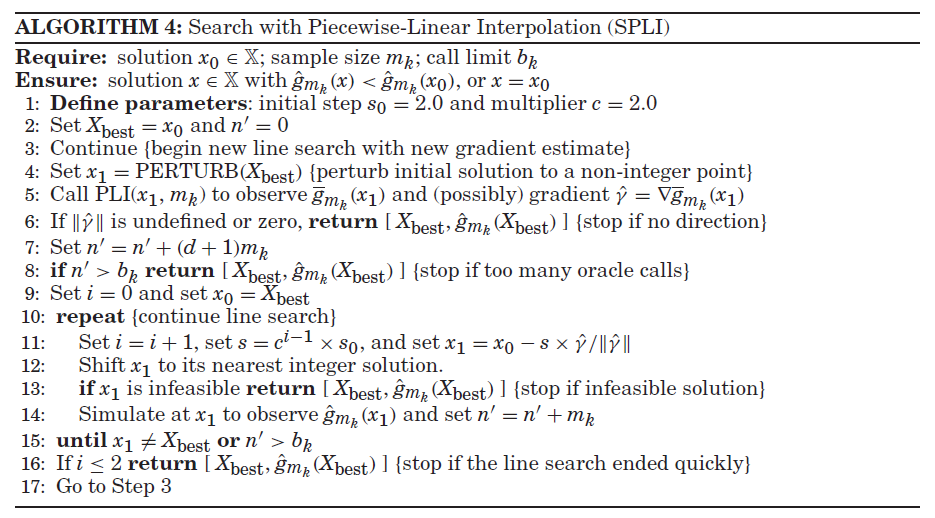
\includegraphics[scale=0.7]{spli.png}
  \caption{SPLI procedure (screenshot from original paper)}
  \label{fig:spli}
\end{figure}

PLI estimates the gradient at a point in the continuous domain by estimating the objective value at all $d + 1$ integer points on the surrounding simplex. Figure \ref{fig:pli} is a screenshot of the PLI procedure from the original R-SPLINE paper \citep{wang2013integer}.The gradient in a given co-ordinate direction is the difference between estimated objective values at opposite sides of the simplex, in that co-ordinate direction. Gradients are normalised when used in the line search. Objective value estimation at integer points, performed in line 8 of the PLI procedure, is done with multiple simulation replications, which could be computationally expensive. Our main suggestion is simple - in this part of the PLI procedure, we replace the multiple simulation replications with a single run of a low-fidelity model. In the homeless care system \citep{burgess2024time}, this low-fidelity model could be a fluid model.

\begin{figure}
  \centering
  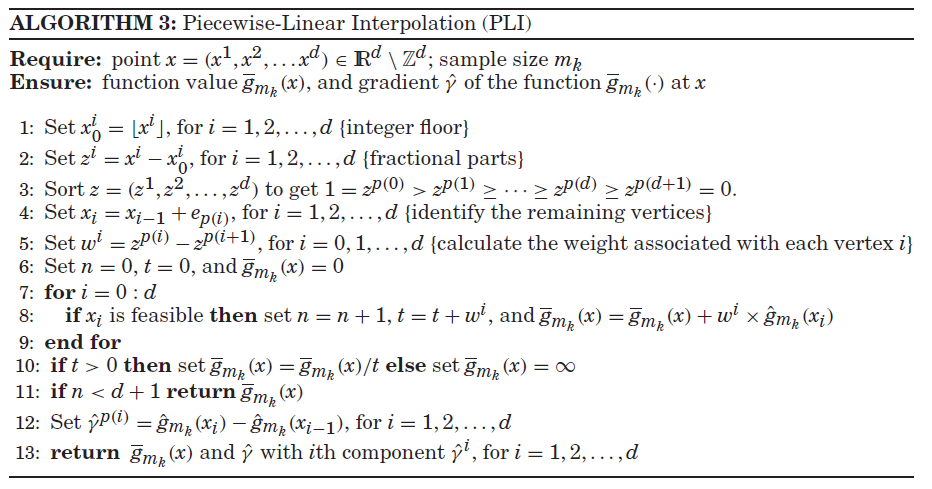
\includegraphics[scale=0.7]{pli.png}
  \caption{PLI procedure (screenshot from original paper)}
  \label{fig:pli}
\end{figure}

We propose the following in case bias in the low-fidelity model leads to poor gradient estimates:
%
\begin{itemize}[noitemsep]
\item At the start of the R-SPLINE procedure, once an initial solution has been set, we could fit a meta model of the objective function response using some initial simulation effort. We could consider a local or a global meta-model. A local model could have the advantage of performing well locally in a focused manner, using for example linear or polynomial terms. The disadvantage of this would be that as we moved around the solution space we would need to regularly refit this model with more simulation effort. A global model may not perform as well locally but may need less simulation effort to maintain throughout the procedure. We could consider a meta-model on the integer-ordered or continuous-valued domain. The former may be more suitable for R-SPLINE (an integer-ordered method) but continuous models such as polynomials or Gaussian process models, may be easier to fit. An appropriate meta model may consist of a `physical' term using a low-fidelity model and a corrective term. \cite{osorio2015computationally} use this idea for a global meta model which weights information from all points on the solution space depending on the distance between those points and the point of searching. As the search continues, the weights change. 
  \item We could use our meta model in PLI (line 8) for objective value estimation at integer points.
  \item During the line search in SPLI (line 14), simulation effort is used to estimate the objective value at new integer points. We could use this information to update or validate our chosen meta model. 
  \item For the first gradient estimation in each SPLI run (first time at line 5), we could obtain two gradient estimates - one using simulation (as in the original R-SPLINE paper) and one with the meta model (as we propose). We could evaluate the quality of the meta model-based gradient estimates and only proceed with it in the given SPLI run if the quality was sufficient.
  \item Another way of validating the gradient information from the meta-model could be to compare the actual change in objetive value with each new solution, to the predicted change from the meta-model based gradient information.
  \end{itemize}

\bibliographystyle{apalike}
\bibliography{bibliography.bib}

\end{document}